\documentclass[11pt,letterpaper]{article}
\usepackage[top=1.00in, bottom=1.0in, left=1in, right=1.25in]{geometry}
\usepackage{graphicx}
\usepackage{latexsym,amssymb,epsf}
\usepackage{epstopdf}

\usepackage{sectsty,setspace,natbib}
\usepackage{float}
\usepackage{latexsym}
\usepackage{epsfig}
\usepackage{graphicx}
\usepackage{amsmath}
\usepackage{array}
\usepackage{lineno}
\newcommand{\R}[1]{\label{#1}\linelabel{#1}}
\newcommand{\lr}[1]{line~\lineref{#1}}
\usepackage{gensymb}
\usepackage{xr-hyper}
\externaldocument{phenncc_supp}
% \usepackage{hyperref}

\usepackage{framed}

\linespread{1.1} % was 1.66 for double-spaced 
% \raggedright
\setlength{\parindent}{0.5in}
\pagestyle{empty}

\parskip=5pt
\pagenumbering{arabic}
\pagestyle{plain}
\setlength\parindent{0pt}

\begin{document}
\begin{flushright}
Version dated: \today
\end{flushright}
\bigskip
\noindent Running title: Tracking \& climate change
% put in your own RH (running head)
\bigskip
\medskip
\begin{center}
% Insert your title:
\noindent{\Large {\bf How temporal tracking shapes species and communities in \\ stationary and non-stationary environments}}\\
% Other titles: `Environmental tracking: It's more complicated than you think' (we hope) 
% or `Environmental tracking: Is it naive? Or, are we just naive?'
\bigskip
\noindent {\normalsize
E. M. Wolkovich$^{1}$ \& M. J. Donahue$^{2}$ }\\
\noindent {\small \it
$^1$ Forest \& Conservation Sciences, Faculty of Forestry, University of British Columbia, 2424 Main Mall, Vancouver, BC V6T 1Z4 (e.wolkovich@ubc.ca)\\
$^2$ Hawai`i Institute of Marine Biology, University of Hawai`i at M\= anoa, K\=an`eohe, HI 96744 (donahuem@hawaii.edu)}\\
\medskip
\end{center}
\noindent{\bf Corresponding author:} see$^{1}$ above; Ph: 604.827.5246 (no fax).\\

\noindent \emph{Authorship statement:} EMW and MJD both conceived of the paper, performed modeling work and edited the paper, EMW additionally wrote the paper and did the literature review, while MJD additionally wrote the supplementary information on the model.  \\
\noindent \emph{Data statement:} Review, so no new primary data, but data from a comprehensive literature review will be archived in an appropriate public repository and the data DOI will be included at the end of the article. \\
\noindent \emph{Keywords:} community assembly, global change, climate change, phenology, environmental variability\\
\noindent \emph{Article type:} Reviews and Syntheses\\
\noindent \emph{Article information:} Abstract: 190 words; Main text: 5,400; Figures: 4; Boxes: 4 (text in Box 1: 343; Box 2: 995; Box 3: 264, Box 4: 738); 115 references (max of 10)
% main text words (5500 without in-text refs approximately) ... boxes can be a max of 800 words 
\newpage
% \linenumbers % If you want to add need to add \begin{linenomath} and \end{linenomath} around all eqns (and check they still show up)
\linenumbers
\begin{abstract} 
% 198 words
Climate change reshapes the environments of all species. Predicting species responses\R{r3misc} requires understanding how well species can track environmental change, and how such tracking shapes communities. Growing empirical evidence suggests that environmental temporal tracking---how an organism shifts the timing of major biological events in response to proximate environmental cues---is linked to species performance and is a structuring force of species and communities today. Here, we review the concept of temporal tracking both in empirical climate change impacts studies and through the lens of community ecology theory.\R{r3misc1} After reviewing how life history theory predicts variation in tracking and trade-offs with other traits, we examine how well competition coexistence theory can be extended to test the current paradigm that climate change should favor species with environmental tracking. We find that existing community assembly theory can be leveraged to  understand tracking in stationary and non-stationary systems and, thus, help predict the species- and community-level consequences of climate change. But it will require greater efforts to integrate priority effects into modern coexistence theory and improved empirical estimates of both fundamental tracking and the underlying cues that shape measures of environmental tracking. 
\end{abstract}
% Finally, we consider how the reality that climate change has widespread effects beyond mean temperature, including shifts in growing season length, variability, and in extreme events, may complicate simple predictions of winners and losers. 
% Limited understanding of organism's phenological cues combined with statistical issues may make many current estimates of variation in tracking less reliable than they appear. Yet these estimates provide the crucial first step to understand variation. 

\newpage
\section{Main text}
Anthropogenic climate change is causing widespread changes in species distributions, with many species shifting in both time and space \citep{IPCC:2014sm,ipcc1point5}. Reports focus on species shifting to higher elevations and poleward \citep{Chen2011} shifting their recurring life history events (phenology)\R{phendefine1} earlier as climate warms \citep{Wolkovich:2012n,cohen2018}, or both \citep{amano2014,socolar2017}.\R{r1ass2} These general trends, however, hide high variability across species. A large proportion of species are not shifting at all \citep{Cook:2012pnas,amano2014}\R{r4misc}, which has raised concerns about whether these species may be more vulnerable to population declines with continued warming. Such concerns come in part from increasing research that links how well species track climate change---especially through temporal shifts---to shifts in biomass, growth and other metrics related to performance \citep{Cleland:2012}. Tracking climate change may then be a major component to understanding and predicting the fitness consequences\R{r3misc2} of climate change, including population declines, with cascading effects on community and ecosystem structure \citep{Menzel:2006xn,Parmesan:2006cr}\R{r1ass}. 

The hypothesis that tracking predicts fitness outcomes with climate change has gained significant traction in the ecological literature focused on global change \citep[e.g.,][]{Cleland:2012} and several areas of theory support it.  Considering tracking as a form of \R{r4misc2}phenotypic flexibility \citep{Piersma:2003wj}, evolutionary models predict species that track will be favored in novel environmental conditions \citep{chevin2010}.\R{r4misc1} Niche models of community assembly suggest that a warming climate should open up new temporal niche space and favor species that can exploit that space \citep{gotelli1996,wolkovich:2010fee,Zettlemoyer2019}.  Yet not all studies find the purported link \citep[e.g.,][]{block2019}, and there has been comparatively little work to improve predictions by formally connecting tracking to community assembly theory.\R{r3misc3}  

This disconnect could be because most ecological theory today is for stationary systems \citep[e.g.,][]{Chesson:1997dz}. While major arenas of research such as `modern coexistence theory' or population ecology are now built on assumptions of a stochastic environment, they generally still assume stationarity, where the underlying distribution of the environment is unchanged across time \citep[i.e., constant mean and variance,][]{barabas2018}. This assumption is common to much of the theory that underlies ecology, evolution, and myriad other research fields \citep[e.g.,][]{Milly:2008yu,nosenko2013}. 

Climate change upends the assumption of stationarity. By causing increases in temperature, larger pulses of precipitation, shifts in snowpack, increased drought, and more storms \citep{ipcc2013}, climate change has fundamentally shifted major attributes of the environment from stationary to non-stationary regimes (see Fig. \ref{fig:climdat} and Box: Environmental variability \& change). This transition is reshaping ecological systems. While new work has aimed to adapt coexistence theory to non-stationary environments \citep{chessonnonstat,volkerass}, there is still little theoretical work on what such a transition may mean for communities and the species within them, despite growing empirical studies.  

\R{aimS}Here, we review the concept of tracking used in the empirical climate change impacts literature and in related ecological theory.\R{aimE} We provide definitions that distinguish between fundamental and environmental tracking, highlighting the distinction between measuring tracking and its fitness outcomes in empirical systems. Then, after briefly reviewing evolutionary theory that predicts variation in tracking across species and environments, we examine how well community assembly theory---especially priority effects and modern coexistence theory---\R{r3misc4}can be extended to test the current paradigm that climate change should favor species that track. 

\subsection{Defining \& measuring tracking}
\emph{Defining tracking}\\
Tracking is a commonly used word in the climate change literature, especially relating to phenology \R{r1ass1}\citep[e.g.,][]{Menzel:2006xn,Parmesan:2006cr,Cleland:2012,deacy2018}. Yet there are few, if any, definitions of it. \R{definetrackS}Conceptual and theoretical treatments of tracking often relate how well an organism matches the timing of a life history event to the ideal timing for that event, what we refer to as `fundamental tracking'. In contrast, empirical studies of tracking often focus on estimating a change in the timing of an event per unit change in an environmental variable, something closer to what we refer to as `environmental tracking'---the change in timing of a major biological event due to an organism's cue system given change in the environment. \R{phendefineS}Both these definitions are readily applied to phenology---the timing of recurring life history events---though they can also apply to non-recurring life history events (e.g., seed germination), or events not normally defined as part of life history.\R{phendefineE}

Fundamental tracking rests on an assumption that there is a timing (an `ideal timing') that yields maximum fitness, and event timings moving away from this ideal result in reduced fitness. \R{r4yardstickS}This is a foundational concept of the trophic mis-match literature \citep{vissergienapp2019}, which often assumes the peak timing of a resource defines the ideal timing for phenological events dependent on that resource \citep[e.g. egg laying dates dependent on caterpillar abundance,][]{Visser:2005bg}. For most events, however, fitness outcomes are likely dependent on a suite of interacting forces \citep[e.g.,][]{reed2013}\R{citeReed}---for example, egg laying dates for migratory birds may depend both on the timing of peak prey abundance and the need to leave nesting grounds before winter.\R{r4yardstickE} Additionally, the timing of events is often connected to the investment process of an event \citep[e.g., number of eggs in a clutch][]{inouye2019}; species evaluate given environmental conditions to detemine both the optimal time for an event that year and how much to invest. Whatever their full underlying causes, fitness consequences of suboptimal timing should drive the evolution of organismal cues to predict and best match the timing of events to the ideal (maximum fitness) timing (the degree of this match defines cue reliability, Fig. \ref{fig:defineET}). These cues combined with environmental variation define what we refer to as temporal environmental tracking (henceforth, `environmental tracking').

\R{moretrackS}Environmental tracking depends on the intersection of the environment's variability---which aspects of the environment vary, how (e.g., temporally each year, spatially at $x$ scale) and how much---and an organism's response to the environment via its proximate cues.  If the varying components of the environment are not in the organism's set of cues, then the organism does not `track' per this definition. \R{Bminusbstart}Environmental tracking at the individual-level is a purely plastic\R{mentionplastic} response to environmental variation \citep[with the plasticity itself an outcome of selection,][]{chevin2010}. At the population-level, tracking may also incorporate evolutionary change in the cue system, depending on both the timescales of study and the species' generation time \citep[this evolutionary response can be predicted as the difference between the environmental sensitivity of phenotypic selection and an organism's plasticity, $|B-b|$ in][]{chevin2010}. \R{itsnotevo}Given our focus on current responses to climate change, we consider environmental tracking here as a mainly plastic response \citep{bonamour2019}, though over longer timescales and in certain systems it should be shaped by selection \citep{franks2012}.\R{moretrackE} 

\emph{Measuring tracking}\\
Measuring `tracking' and comparing variation in it across species, space and time is a rapidly growing area of ecological research \citep[e.g.,][]{Cook:2012pnas,fu2015,thackeray2016,cohen2018}. Studies estimating fundamental tracking are uncommon \citep[but see][]{visser2006,charm2008}, given in part the difficulty of measuring fitness, though many studies in the synchrony literature attempt to link consumer change to resource change, with an assumption that the resource is the dominant determinant of ideal timing for the consumer \citep[though this may rarely be true, see][]{Singer:2010eb,Johansson2012, reed2013}\R{citeReedagain}.  Instead, most studies focus on estimating something akin to environmental tracking. Some studies estimate simply change in days over time \citep[e.g.,][]{Parmesan:2007tv,kharouba2018}, though most studies now estimate shifts in response to temperature \citep[for example, multiple meta-analyses show plants' spring phenology shifts with spring or annual temperatures 4-6 days/$\degree$C on average across species,][]{Richardson:2006qh,Wolkovich:2012n,thackeray2016} or precipitation \citep{inouye2002,Craine:2012kl}. % In many studies environmental tracking is estimated as the slope of phenological event dates regressed against environmental metrics hypothesized to link to underlying cues, though this estimate will be more or less accurate depending statistical limitations and current knowledge of an organism's cue(s) \citep{chmura2019}.

All species-rich studies of phenology-climate relationships find high variation \citep{Cook:2012pnas,thackeray2016}, including some species that do not track or track poorly (i.e., high noise surrounding observed statistical relationships). Researchers have worked to link such variation to the underlying cues \citep[e.g.,][]{Cook:2012pnas}, species traits \citep[e.g.,][]{cohen2018} and trophic level \citep[e.g.,][]{thackeray2016}. These approaches hint at the three majors classes of reasons that underlie species that do not appear to track climate or appear to track poorly: (1) species do not track, as environmental tracking may either not be possible or optimal for all species \citep{simons2011}, (2) lack of firm biological understanding of the cues that underlie tracking \citep{chmura2019}, and (3) statistical artifacts that make it difficult to measure tracking robustly (see Box `Challenges \& opportunities in measuring tracking'). 

Limited understanding of organisms' phenological cues combined with statistical issues may make many current estimates of variation in tracking less reliable than they appear. This in turn makes robust quantitative analyses across species difficult \citep{brown2016,kharouba2018}, yeilding a muddy picture of which species, when, and where, do and do not track. Given this difficulty, we believe clear testable predictions from ecological theory are especially critical to guide research today \citep{Smaldino2016}.  

\subsection{Tracking in single-species environments}
% \subsection{Understanding variation in environmental tracking} % Plasticity tells us when it would be beneficial in timing to changing environments; when evolution it acts through a cue system which is selected for via OPT. 

\emph{Predicting variation in environmental tracking in stationary systems}\\ 
Considering environmental tracking as a plastic trait \citep[e.g.,][]{charm2008,nicotra2010,forsman2015,inouye2019} evolutionary models predict strong selection for tracking in heterogeneous environments where there are predictable cues for the ideal timing of events and the underlying genetics to develop a heritable cue system \citep{Piersma:2003wj,reed2010}. Tracking is likely strongly heritable, given that many phenological cues are themselves strongly heritable \citep[e.g.,][]{vanAsch2007gcb,Wilczek:2010ad}. \R{r1consS}Selection, however, can be lower than expected from reaction norms predicted by simple models of plasticity for many reasons, including unavoidable trade-offs with tracking \citep{Singer:2010eb,Johansson2012}, gene flow from other environments that may continually push a population away from its local optimum \citep{lenormand2002}, limits due to standing genetic variation  \citep{Franks:2007wd,ghalambor2015}, or deeper evolutionary history that may produce co-evolved traits making it difficult for selection to act solely on tracking \citep{Ackerly:2009ly}.\R{r1consE} 
% MJD: This reads well.  I feel like there shoudl be more emphasis on the `predictable environment' part, as the relatinship to tracking is clear: particularly for irreversible plastic traits like many of traits for phenological timing, the availability of envt'l cues that could predict the best timing of event is critical.  Such an environmental feature has to exist at an appropriate timescale for the trait in question, in addition to the fact that you have to be able to select on the ability to measure that environmetnal feature.  

These constraints form one part of the formula for predicting the cue system species should evolve, with the costs and benefits of cues being the other main components \citep{donahue2015}. The cost of cues includes the machinery an organism uses to monitor its environment (e.g., accumulated temperature or daylength), while the benefits are the increases in fitness gained from better timing (e.g., how much tissue is saved by avoiding a coldsnap).  Apparently poor cues may occur for organisms in environments where there is both a low cost and low benefit to the cue(s). Similarly, expensive cues, such as complex multivariate ones, are possible given a high pay-off. Most in-depth studies of species' phenological cues find evidence for complex multivariate ones \citep{chuinearees}. These cues almost always appear adapted to handle unusual---though not completely uncommon---years when the simple cue alone would fail (that is, would trigger growth, reproduction or another life history event at a suboptimal time), suggesting that multivariate cues may provide a large benefit in best coupling the timing of cues to the ultimate controls (i.e., cues that couple environmental tracking strongly to fundamental tracking). \R{plasE}
% Constraints can arise from the organisms itself or from its environment.  Organismal contraints include the availability of machinery to track the environment as well as other fundamental differences in life history---for example, the type and amount of loss an organism can sustain each season is limited by its generation time and other attributes related to long-lived lifestages that yield buffered population growth \citep{Chesson:1997dz}.  Enviromental constraints include the fundamental predictability of the enviornmnet:  are there early season environmental variables that can predict later season phenomena? 

\R{bhS}Tracking should generally not be favored in unpredictable environments, or environments where species otherwise face high uncertainty in the timing of investment decisions; instead theory suggests the optimal strategy may often be to bet-hedge \citep{Venable:2007os,donald2013,decasas2015}\R{r1ass4} via a high diversity of timings or one conservative timing. Because bet-hedging, by definition, maximizes geometric-mean fitness in the long-run, its short-term outcomes can appear maladaptive. How often observed `maladaptations,' which may easily include species that do not track or appear to track poorly, are actually the outcome of bet-hedging is difficult to estimate, as robustly assessing bet-hedging requires studies of fitness over longer timescales than many current field experiments \citep{simons2011}.\R{simonsref1}

Environmental variation often includes both predictable and less predictable aspects. In such cases theory predicts organisms may evolve tracking that is a mixed strategy between bet-hedging and plasticity \citep{wong2005}. Taken together, life history and related evolutionary theory provide multiple reasons species may not track or track weakly, suggesting that---at least in stationary systems---we should expect a number of species that do not track.\R{bhE} \\

\emph{Predicting variation in environmental tracking in non-stationary systems}\\
Expectations from life history theory of which species should track are generally based on assumptions of stationarity, thus a major open area of research is adapting life history theory to non-stationary environments. Multivariate cues may be especially robust to a non-stationary environment if they provide a tight coupling of cues to fundamental tracking, and that coupling is maintained in the non-stationary environment \citep{dore2018}. But multivariate cues may equally be most vulnerable to failure if non-stationarity decouples the cues from fundamental tracking \citep{bonamour2019}. \R{r3birdsS}For example, consider an organism's whose cues evolved based on a correlation between peak prey abundance and daylength: the daylength cue that could be reliable in a stationary environment (generally predicting preak prey abudance based on daylength, with some interannual variation), but would become unreliable if warming continually advances peak prey abundance. Predicting the outcome of non-stationarity would be possible from the stationary environment in this case given researchers know (1) the full cue system of an organism, (2) how it relates to fundamental tracking, and (3) how both that cue system and the underlying fundamental model shift with non-stationarity.\R{r3birdsE}

In recent years, plasticity theory has developed to provide insights on non-stationarity \citep[or `sustained environmental change,' see][]{chevin2010}. Models of the role of plasticity in novel environments provide an important bridge to understanding the outcomes of non-stationarity, generally predicting non-stationarity should favor highly plastic species. This outcome, however, assumes there are no costs related to plasticity \citep{Ghalambor2007,tufto2015}. If there are costs associated with tracking, then species may evolve lower tracking, because it should trade-off with other traits \citep{auld2010}. 

\subsection{Tracking in multi-species environments} 
Life history theory that may help predict tracking often ignores other (non-focal) species or abstracts them as an aspect of the environment. While the trophic mis-match literature has addressed this gap for trophic interactions \citep{Visser:2005bg,vissergienapp2019}, these is little consideration of competitive coexistence, yet this perspective is critical to understanding environmental tracking \citep{metcalf2015}. Considering selection in multi-species environments structured by competition highlights that tracking cannot be considered as a singular trait, but must be evaluated as part of a trait syndrome \citep[or mosaic of traits,][]{Ghalambor2007} and should ultimately produce communities of species where tracking trades-off with other traits. 

As tracking often relates to the timing of a resource pulse, traits related to resource acquisition are likely contenders for a trade-off. Species with traits that make them poor resource competitors may need to track the environment closely to take advantage of transient periods of available resources, but will risk tissue loss to harsh environmental conditions more prevalent early in the season (e.g., frost or snow) and thus may need to be more stress tolerant.\R{r1stress} In contrast, species with traits that make them superior resource competitors may perform well even if they track environments less closely, because their resource acquisition is not strongly constrained by competitors. Examples include under-canopy species leafing out earlier to gain access to light \citep{heberling2019} or species with shallow roots starting growth sooner in an alpine meadow system, while species with deeper roots begin growth later \citep{Zhu2016BioLetters}. In such cases, tracking is akin to a competition-colonization trade-off \citep{Amarasekare:2003tq}, where species that track well gain priority access to resources and, thus, may co-exist with superior competitors. Research to date supports this, with several studies linking higher tracking to traits associated with being poor competitors \citep{Dorji2013,lasky2016,Zhu2016BioLetters}. Further, many studies have found a correlation between higher tracking and `earlyness' each season, which has been linked to resource acquisition traits associated with lower competitive abilities \citep[][see Box `Trait trade-offs with tracking']{wolkovich2014aob}.  

Understanding these trade-offs is clearly critical, but understanding the short-term dynamics of a changing environment with plastic species is additionally important and highlights how little ecological theory we have for tracking. While evolutionary theory sometimes predicts the outcome of a new environment, non-stationarity in the climate today means understanding the trajectory to that outcome may be most relevant---and bridges across evolutionary and ecological timescales. Evolutionary models show how plasticity may limit standing variation and thus reduce fitness in novel environments \citep{Ghalambor2007,fox2019}. But whether such findings extend to systems transitioning from stationary to non-stationary will likely depend on how non-stationarity affects the rate of adaptation \citep{chevin2010}, and how ecological shifts reshape the environment. Efforts to model expected outcomes given climate projections and current understanding of plasticity and genetic variation underlying event timing in some organisms provide the empirical start to this \citep[e.g.,][]{fournier2016}, but more eco-evolutionary models that bridge this gap may prove especially useful. 

\emph{Including tracking in multi-species community assembly models} \\
Predicting how tracking may determine which species are effectively winners and losers with climate change requires integrating non-stationary environments into models of community assembly. Recent advances in coexistence models, sometimes called `modern coexistence theory,' recognize that both mechanisms independent of fluctuations in the environment (e.g., R* and other classical niche differences) and mechanisms dependent on fluctuations in the environment (relative non-linearity and storage effect) can lead to coexistence \citep{Chesson:1997dz,Chesson:2000vd}. These models, which underlie much of current community ecology research \citep{Mayfield:2010fe,barabas2018,ellner2019}, provide a framework to begin to model environmental tracking and non-stationarity. 

How the environment is defined in most community models falls into two broad categories. In some models the environment is expressed as variation in parameters related to species. For example, in many lottery models the environment appears, effectively, as variation in birth and death rates. Building a changing environment into such models thus requires knowing how environmental shifts filter through to species-level parameters \citep{Tuljapurkar2009}. For example, \citet{volkerass} added the temporal environment to competition models by defining interaction strength as dependent on the temporal distance between species. This is somewhat similar to models that include \R{doublethe}the environment effectively through different levels of asynchrony \citep[e.g.,][]{Nakazawa2012,revilla2014}. In other models, the environment is more specifically defined. Many of these models define the environment as a resource (e.g., many seed germination models that begin with a resource pulse each year), and thus generally model something close to fundamental tracking. 

Models that explicitly include the environment provide a major opportunity to predict how environmental tracking and non-stationarity determine future communities. As an example, we modeled  a shift to earlier growing seasons using a common coexistence model. The shift to earlier seasons favored species that could track, increasing their prevalance by shifting a modelled trade-off between tracking and competitive ability (via $R^*$), see Fig. \ref{fig:modelfig} and Box: `Adding tracking and non-stationarity to a common coexistence model'). Like all models, it rests on a number of assumptions, including that species' cues remain as reliable in the stationary as non-stationary environment, but shows how non-stationarity could benefit trackers. 

Most current models (including the previous example) examine the environment from only one of two relevant angles: they represent the environment as used for species' cues (e.g., many models of plasticity) or they represent the environment as directly affecting fitness (e.g., the storage effect model). Combining these two angles may be especially critical to understanding the costs and benefits of tracking in non-stationary environments. 

Layered onto the different angles that different models take on the environment is how species responses to the environment are defined. In general, species responses to the (resource) environment can be broadly grouped into models that explicitly define when species start an event (e.g., spawning or germination) in response to the environment versus those that model the magnitude (e.g., the number of propagules or seeds) of response to the environment. Models that explicitly include when a species starts an event are often focused on situations where order of arrival is critical to predicting coexistence outcomes. For example, models of priority effects through niche pre-emption highlight the advantage tracking may provide when it allows species to be early (and when there is no cost to being too early): early arrivals receive a head-start advantage, by gaining priority access to resources (the environment) they can draw down the resources available to later arrivals \citep{fukami2015}. Such models predict the early-arriving species to out-compete other species, unless the order of arrival varies by year or there are trade-offs with other species' traits (see Fig. \ref{fig:conceptmodels}).

Other models canalize species' responses to the environment into production and investment. For example, most models of inter-annual competition \citep[most explicit examples of `modern coexistence theory,' e.g.,][]{Chesson:2004eo,Angert:2009} fall into this camp. Species produce (via offspring, tissue etc.) differentially depending on the environment each year and outcomes are mediated through density. While these models superficially may seem disconnected from timing, they critically highlight how event timing often relates to production and, thus, investment across years. Further, they almost always model the environment as a distribution (see Fig. \ref{fig:conceptmodels}), which provides the opportunity for the environment to alter the competitive environment each year and, thus, structure coexistence. 

Storage effects models explicitly characterize the environment filtered into species through low density per capita growth rate ($E_i$), and thus highlight that understanding how environmental change impacts low density per capita growth rate can yield predictions of future communities: if non-stationarity in the environment affects $E_i$ in such a way that it decreases the covariance between the $E_i$ and competition ($cov(E_i, C_i)$), it will decrease the storage effect as a means of competitive coexistence.  However, this leaves an enormous research program to understand how the changing environmeny---i.e., the changing joint distribution of key environmental variables---filters into the per capita low density growth rate of individual species and competiting suites of species.

A model where species vary both when they start an event and how much they produce dependent on the environment would capture the important attributes of tracking---combining head-start advantages from being early with production variation based on the fitness of the environment. To our knowledge, however, most models approach these questions separately, though models of bet-hedging come closest \citep{Gourbiere2009,tufto2015}. A model that explicitly includes the linked decisions of when to time an event and how much offspring/tissue to produce during the event could provide fundamental insights on the relative importance of each aspect of this process. Such a model could be adapted to address multiple questions of environmental tracking, including how these decisions (`when' and `how much') may trade-off and which other traits may be most strongly linked to tracking, as well as explicitly modeling the costs and benefits of tracking in stationary systems---a critical precursor to extending it to non-stationary systems. 

Extending models to non-stationary systems is crucial to testing how environmental tracking relates to species persistence with climate change, and research has already begun to tackle this non-trivial challenge \citep{chessonnonstat,legault2019,volkerass}. Most work to date, however, focuses on conclusions from systems that are intiatilized as non-stationary, ignoring the transition between stationary and non-stationary. Yet we expect this transition may be most critical because communities formed in stationary environment periods (or periods with environments lower non-stationarity) are effectively filtered and assembled by that environmental regime and thus produce the baseline of variation and assembly dynamics for a shifting environment. While analytical solutions for systems transitioning from stationary to non-stationary may take time to develop \citep{chessonnonstat}, simulation work can provide an immediate intuition and framework to address this challenge (for an example, see Box: Adding tracking and non-stationarity to a common coexistence model). 

Outcomes for such community assembly models also depend on how effectively closed communities are  (i.e., without dispersal or evolution). Dispersal of species or individuals with traits that make them better matched to the non-stationary environment would lead to new communities that may persist or be continually re-assembled as long as the environment remains non-stationary. Indeed, this logic underlies the argument that invasive species may be superior trackers benefiting from how climate change has altered growing seasons \citep{Willis:2010al,wolkovich:2010fee}. Evolution equally could alter predictions by allowing species traits to evolve in step with environmental change. Long-term population \citep[e.g.,][]{colautti2017} and resurrection studies \citep{wilczek2014,yousey2018}, as well as field experiments \citep{colautti2017,arab2019}, have repeatedly shown species can shift to earlier flowering times, higher thermal tolerances or related genetically-controlled traits that confer higher fitness in warmer climates. Yet these studies also highlight that responses can be lagged \citep[e.g.,][]{wilczek2014}, associated with reduced population viability \citep[e.g.,][]{colautti2017}, or other factors that may constrain adaptive responses, making understanding the competitive outcomes of the community assembled before environmental change critical. 

\subsection{Future directions}

Growing empirical research highlights that environmental tracking is linked to species performance and, thus, may be critical to understanding the forces that assemble communities and determine species persistence, especially as anthropogenic climate change is reshaping the environment of all species. We have outlined above how  current community ecology theory could make advances relevant for the Anthropocene, specifically through models that combine effects of variation in timing and production amounts and models that include environment as impacting species' cues, as well as species' fitness. Such models would explicitly allow the potential costs and benefits of tracking  depending on how closely environmental tracking matches fundamental tracking. But to best test and develop such models we need a greater understanding of how the environment is changing, more robust estimates of environmental tracking and how it fits within a mosaic of other correlated traits. 

\emph{How is an organism's environment changing?} \\ 
Currently, much research has focused on one major shift in the climate system (earlier growing seasons), but research on multivariate environmental shifts is growing and will be critical to understanding how climate change affects an organism's whole environment. Ecologists can guide these efforts by identifying environmental shifts that are often linked. \R{r3misc5}For example, warming temperatures may drive earlier seasons and higher evaporative loss of some resources such as water. Researchers can also aim to more consistently and fully characterize the environmental distributions of their systems that appear to drive species performance and interactions: the environment of the years of study should be clearly reported and compared against long-term and recent climate for each system. 

More interdisciplinary research with climate science could also speed a fuller understanding of what shifts are and are not expected with climate change, and what climate variables are inherently correlated. Such correlations make estimating cues and other biological parameters from long-term data especially precarious \citep{tansey2017}. But these correlations are equally critical in considering how species may view their environment and whether environmental change will couple or uncouple links between proximate cues and fundamental tracking \citep{bonamour2019}. \\

\emph{Understanding and measuring `tracking'} \\
Understanding how the environment is changing represents just one step towards robust measures of environmental tracking. Shifting environmental regimes must then be filtered through species cues, and impacts on growth and survival. Studies should clarify their definition of tracking, how the environment is defined, how an event relates to fitess, and how well---or not---the underlying cue system is understood (see Box: `Challenges \& opportunities in measuring tracking'). Currently, many studies examine fundamental and environmental tracking at once \R{r3misc6}\citep[e.g.,][]{visser2006,charm2008,Cleland:2012,yang2020}, which is clearly helpful in advancing the field. However, the more researchers can clarify when and how they are addressing fundamental tracking versus environmental tracking, the more easily we can compare results across studies. We expect progress will come from a balance between measures of fundamental tracking (measuring both event date variation and fitness), estimating an organism's system of cues (generally through controlled experiments followed by tests in the field), and measuring the change in an event date from environmenatal variation that is due to cues (environmental tracking). \R{r4miscvague} Clear statements of what is and is not known and measured will help.

\emph{What major traits trade-off with tracking?} \\ 
Basic theory of plasticity and competition suggest that environmental tracking must trade-off with other traits to allow multi-species communities. Yet to date empirical work has mainly documented tracking, linked it to performance, or focused on how it varies between native and non-native species \citep{Willis:2010al,wolkovichAmBot2013,Zettlemoyer2019}. Such work lays the groundwork that environmental tracking is important, but future empirical research should address how this trait co-occurs with other traits. Research has highlighted some traits that co-vary with tracking \citep[e.g.,][]{kharouba2014,lasky2016,Zhu2016BioLetters}, but to tie this empirical work to models requires more research on traits that link clearly to theory, and a fuller understanding of how tracking and other traits jointly contribute to performance under varying environments. 

Traits that link to resource competition, as we focus on here \citep[as others have as well, see][]{volkerass}, may be especially fruitful for greater research, but should not be the only ones considered. For example, traits related to predator tolerance or avoidance may also play a role, but have been effectively unstudied.  As empirical research in this area grows, models can aid progress in understanding the outcomes of these trade-offs for community assembly. \\ 


\subsection{Stationarity in the future}
While most environments today are climatically non-stationary and have been for decades, the climate will return to a more stationarity form in the future. There are many possible pathways to climatic stabilization, but almost all require first the stabilization of greenhouse gases---the subject of much policy and political debate. Once greenhouse gas emissions stabilize climate will not quickly snap back to a new stationary phase. Instead systems will slowly approach a new climatic stationarity depending on how they are effected by the earth's multiple thermal reservoirs, and, in turn, how quickly those reservoirs stabilize. The timescale of this approach is generally expected to be on the scale of centuries, but could be much longer in certain oceanic systems \citep{ipcc2013ch12}. Thus, ecologists are---and will remain for the foreseeable future---in a research area structured by climatic non-stationarity. 

As paleobiologists and evolutionary biologists often point out, climatic nonstationarity is a common part of the earth's history \citep{Jansson:2002nz}---even if stationary periods---be they cold or warm (glacial and interglacial periods), or dry or wet (e.g., megadroughts or pluvials)\R{r2precip1}---are more common. Indeed, while much of this work has examined how species survive for millions of years given large oscillations in climate \citep{provan2008}, the periods that provide the most dramatic community reshuffling are periods shifting from stationary to non-stationary climate regimes \citep{vrba1980,vrba1985}. Such stories of the past are now fundamentally happening today, and ecology is challenged to understand how transitions between stationary and non-stationary environments are reshaping the species and communities we have today and will in the altered climates of our future.\R{r2precip2}


\section{Acknowledgments}
We thank I. Breckheimer, D. Buonaiuto, E. Cleland, J. Davies, G. Legault, A. Phillimore and three anonymous reviewers for helpful comments that improved the manuscript, K. Slimon for help with trade-offs review, and the NSERC Discovery Award (RGPIN-05038 to EMW) and Canada Research Chair in Temporal Ecology (EMW) programs that provided funding. 

% Chapter 12 of IPCC WG1 "Long-term Climate Change: Projections, commitments and irreversibility" (Section 12.5: Climate Change Beyond 2100, Commitment, Stabilization and Irreversibility)

% Note to self: environmental tracking seems used by spatial folks ...
   % https://www.nature.com/articles/srep36265
% But! The temporal autocorrelation folks use it too ... this is mainly one-site population work I think and pretty damn similar to our use!
   % https://royalsocietypublishing.org/doi/10.1098/rspb.2011.0487 (2011)
   % https://link.springer.com/article/10.1007/s12080-015-0276-6 (2016)
   % https://besjournals.onlinelibrary.wiley.com/doi/full/10.1111/1365-2745.12077 (2013) 
% And this annual review has a whole section (no definition though that I saw):
   % https://www.annualreviews.org/doi/full/10.1146/annurev.ecolsys.35.120202.110110 ... about fossil 'The principal cause for these patterns appears to be species-, and perhaps clade-level, environmental fidelity that results in long-term tracking of physical conditions. ... biotas do appear to track climates, but such tracking is certainly influenced by geographic and physicochemical barriers' 
% So I say it is all the same thing! And we focus here on the temporal aspect .... give nod to space at the end of ms maybe?


%%
%%
%%
%%
%%

% We believe robust comparisons of tracking metrics require more efforts to estimate the full suite of cues species use, or at least bracket its uncertainty, then connect it to environmental variability and what aspects of the environment the researchers have measured. Yet estimates likely capture important realities of environmental tracking. 

\newpage
\section{Boxes}

\subsection{Box: Environmental variability \& change} % 348 words
Decades of ecological research highlight how temporally variable environments shape species and their communities at multiple scales \citep{Sale:1977oq,Chesson:1997dz}.  In seasonal landscapes, the environment limits periods for growth each year (e.g., by temperature or drought); within-year variability in the environment (e.g., daily, hourly or finer resolution temperatures or rainfall amounts) compounds into inter-annual variability that shapes the distribution of the start and end of growing seasons. For long stretches of history this variability has been effectively stationary; that is, the underlying probability distribution that describes the start (or end) of the season (e.g., the date of the last major frost) does not change, even though the date may be dramatically different from one year to the  next. % The shape of this underlying distribution varies across systems and in how it is measured---for example, the total amount of rainfall across years in semi-arid systems is often highly skewed (rare high rainfall years, with many more below-average rainfall years) compared to the more normal (Gaussian) distribution of the thermal sum of temperate growing seasons. 
% In seasonal landscapes, periods for growth each year are limited (e.g., by temperature or drought), and species must manage within-year variability by timing when to grow and when to reproduce \citep{donohue2002}. 

In other time periods, variability has been non-stationary in one or multiple dimensions. For example, climate in the northern hemisphere includes long warming and then cooling periods (i.e., increasing then decreasing means of the probability distribution) at the start of the Holocene, when the earth was coming out of the last glacial maximum. Anthropogenic climate change is a similar non-stationary process, with warming evident around the globe and knock-on effects for other climate metrics, such as heat extremes and the size of precipitation events. % While only several decades ago, ecology was focused strongly on stochasticity in stationary systems \citep[e.g.,][]{Ripa1996,Kaitala1997}, climate change has shifted the focus to understanding stochasticity in a non-stationary framework \citep[e.g.,][]{cazwavelets,ehrlen2016,legault2019}.

Understanding non-stationarity in ecological systems requires first identifying which aspects of the environment have shifted---and how they have shifted with respect to one another---as the underlying  distributions transition from stationary to non-stationary (Fig. \ref{fig:climdat}). For example, with climate change, warming has increased mean temperatures over time, with minimum temperatures generally increasing more than maximum---this results in an underlying distribution for daily temperature where the mean is increasing through time while the within-day variance is decreasing \citep{ipcc2013,screen2014}.  Understanding the impacts of climate change further requires recognizing that most systems can be considered stationary or non-stationary depending on the timescale and period of study. Thus, predicting the consequences of current non-stationarity in ecological systems benefits from identifying the type and scale of non-stationarity, relative to long-term trends.  



\subsection{Box: Challenges \& opportunities in measuring tracking} % 820 words ... NEED to cut at least 30! Analyses of long-term observational data are also the most at risk of interpreting statistical bias or artifacts as biology.
Increasingly, research has outlined statistical difficulties in measuring tracking, which may underlie many observations of species that do not track. These issues mostly relate to the challenges of observing phenological distributions \citep{steer2019,carter2018} using discrete (calendar) time, low power, and the complexity of climate data. 

Non-stationarity in units comes in many forms---estimates of mean days shifted per decade depend on the climate of the decade(s) studied, which is not consistent in many systems \citep{Ault2011,McCabe2012}. Estimates based on a relevant climate variable can sometimes ameliorate this problem, but may be equally vulnerable to non-stationarity in units \citep[e.g.,][]{Sagarin:2001fu}. For example, processes that depend on thermal sums reported as days/$\degree$C will generally appear to decline with warming, as the thermal sum of an average day has increased in most regions with climate change. Relatedly, estimates of long-term change using simple linear regression depend on the climate at the start of the time-series (with greater changes seen from time-series that started in unusually cold decades, such as the 1950s for much of North America). 

Low power is widespread in ecology, where even `long' time-series may be far too short for robust analyses \citep{bolmgren2013,kharouba2018}. Authors should be especially cautious if they find only large effects appear significant \citep[e.g.,][]{CaraDonna2014}, which is a well-known statistical bias associated with p-values \citep{loken2017}. Additionally, effect sizes that are higher when climate variability is higher (for example, in temperate habitats temperature is highly variable in the spring and autumn compared to summer) may be more related to variation in statistical power than to biology. 

Most of the outlined statistical issues can be addressed by improved statistical approaches \citep[e.g.,][]{gienapp2005,pearse2017}, though such approaches may uncomfortably highlight how uncertain many current estimates are \citep{brown2016}. Impacts of start-years for long-term time-series can be muted by applying change-point or hinge models \citep[e.g.,][]{kharouba2018}, while metrics that move away from calendar time (e.g., day) can help address non-stationarity in units.  We suggest mixed models should be used more widely alongside randomization and/or data-simulation approaches \citep[e.g.,][]{bolmgren2013,kharouba2018} to better estimate and communicate uncertainty in studies \citep{pearse2017}. And researchers should identify what results bias may produce. For example, growing evidence suggests a potential fundamental trade-off where early species track and possess a suite of traits to related to faster growth and shorter lifespans, while later species track less and possess traits related to slower growth and longer lifespans---these later species may bet-hedge more given their longer investment window. This, however, could equally be an artifact where early species use simpler cues, and, thus, their tracking is measured more accurately given current methods.

Even without statistical issues, translating phenological and climate data into estimates of tracking requires a firm biological understanding of an organism's cues, critical knowledge that researchers rarely have \citep{chmura2019}. Currently, `tracking' is often measured simply as the relationship between the dates of the phenological event and a simple abiotic metric, such as mean monthly temperature. Simple environmental metrics, however, are almost always proxies for a more complicated underlying physiology where simple cues---such as warm temperatures---can be modified by other cues, such as photoperiod, drought or light spectra \citep{Bagnall1993,Stinchcombe:2004ec}. Teasing out these other cues, however, generally requires nuanced approaches to observational data with explicit assumptions \citep{tansey2017}\R{citetansey} or controlled experiments \citep{Wilczek:2009oa,Caffarra:2011qf}. 

Modeling multivariate cues well is inherently difficult \citep{chuine2016}, especially since one cue may dominate in many conditions. For example, woody plant leafout responds to warm spring temperatures, but also to cool winter temperatures to prevent leafout in mid-winter warm snaps that occur long before the last frost. Often this cool-temperature effect may be masked by sufficiently cool conditions. With warming from climate change, however, this additional trigger---which appears to vary by site, species and even inter-annual conditions \citep{dennis2003}---may become critical \citep[and potentially lead many phenological models to fail spectacularly in the future as additional cues come into play, see][]{chuine2016}. Tracking in species with longer generation times may be especially complicated, as species may track low frequency climate signals and make investment choices on far longer timescales than species with shorter lifespans \citep{morris2008}. In some semi-arid systems, species time growth to pulses of rain, but only when those rain events occur with cooler temperatures that indicate the start of the rainy season, and not a rare summer rainfall event in the middle of months of drought \citep{Wainwright:2012tw,wainwright2013}. 

Addressing these issues is possible if more researchers build a model of their species' cues (embrace your inner physiologist, or collaborating with one) and interrogate it. Defining the framework under which we expect cue systems evolved or works (e.g., bet-hedging) then testing how well it works, and where it fails \citep[see][for an example]{johanOCR}, could yeild rapid progress. Model interrogation also helps embrace the contradictory pulls of conducting experiments to identify mechanistic cues and how they are filtered through the multivariate climate of the real world. But we lack the suites of experiments, which build from identifying cues to understanding how they act when correlated, for most organisms \citep[but see][]{Wilczek:2010ad,Wilczek:2009oa}.


\subsection{Box: Trait trade-offs with tracking} % 264 words
% Supp figure is still not showing -- comes up with ?? in Figure reference.
Research on phenological tracking and traits has increased greatly in recent years, with a major uptick in studies after 2010 (see SI Fig. \ref{fig:papertrends}). Most papers examining tracking and other traits across species have focused on plants (20/30), followed by birds and Lepidoptera (both 4/30), plankton and aphids (both 1/30). The most studied trait was how early or late a phenophase occurred (e.g., date of flowering of start of migration for a species, termed `earlyness' by some authors), with earlier species tending to track more \citep[studies included both birds and Lepidotera,][]{Diamond:2011nx,Ishioka2013,kharouba2014,jing2016,du2017}. While this is an important link, it is vulnerable to statistical challenges (see Box `Statistical challenges in measuring tracking'). Few studies examined whether tracking correlates with resource acquisition traits; those that did generally found species with higher tracking also had traits associated with lower competitive abilities under low resources \citep[e.g., being shallower or lacking a taproot rooted][]{Dorji2013,lasky2016,Zhu2016BioLetters}. These species were often also early \citep[e.g.,][]{Dorji2013,Zhu2016BioLetters}, suggesting tracking may relate to a syndrome of traits that allow species to be rapid colonizers each season, but poor competitors for resources. Indeed, previous work has documented that species with earlier phenophases tend to have resource acquisition traits associated with lower competitive abilities \citep[e.g., they tend to be of lower height, have shallower roots, narrower diameter vessels, thinner leaves, and grow faster, reviewed in][]{wolkovich2014aob}. % See \cite{kimball2012,huang2016} as contrast....
% need to add Jing2016 to "studies included both birds and Lepidotera"

\subsection{Box: Adding tracking and non-stationarity to a common coexistence model} % 776/800 words now
To understand the role of environmental tracking by species in variable environments we use a simple model that allows within- and between-year dynamics to contribute to coexistence. As the model is akin to many commonly used seed germination models \citep{Chesson:2004eo}, we follow a similar terminology for ease; however the basic structure of our model could apply to other systems with one dominant (non-renewing)  pulse of a limiting resource each season (e.g., water from rain or snowpack),\R{r2precip} or a multivariate resource pulse that acts effectively as one resource (e.g., nitrogen and light drawn down together over the season). In this model the environment is included between-years via variable germination, and within-years the environment is explicitly included as a resource pulse at the start of the season. We adjust the biological start time of species ($\tau_i$ for species $i$) to also allow species to respond to the environment dynamically through what we refer to as tracking. Here, tracking effectively moves a species intrinsic start time closer to the environmental start time in that year, resulting in a higher germination fraction (see SI for complete description and equations).

Species can co-occur via equalizing mechanisms, but they require stabilizing mechanisms to coexist. Species that is, cannot coexist given only variation in tracking---coexistence requires variation in another trait axis. As theory and empirical work suggest this trade-off may involve traits related closely to resource competition, we varied species' $R^*$. With variation in tracking and in $R^*$ species can persist together as long as those species with a temporal niche advantage are also the inferior competitors (Fig. \ref{fig:modelfig}). That is, species that can draw resources down to a lower level and are thus the superior within-season resource competitors (lower $R^*$) can persist with species with that are inferior competitors but have realized biological start times closer to the environmental start time---a finding inline with currently observed empirical trade-offs (see Box `Trait trade-offs with tracking'). These trade-offs, however, are all environmentally dependent. They hold only so long as the environment is stationary. 

We examined how trade-offs may be transformed by a non-stationary environment, by transitioning a stationary environment---in which two-species communities had persisted for 500 years---to non-stationary, via an earlier start of season (earlier timing of the resource pulse, $\tau_p$, Fig. \ref{fig:modelfig}; see SI for more details). By changing a fundamental niche axis (the distribution of the environment, an axis along which these communities were structured), we shifted one major part of the trade-off: the new non-stationary environment favored an earlier start time than the previous stationary environment. This, in turn, reshaped our two-species communities, which depended on this trade-off for persistence. 

While the non-stationary environment favored higher trackers (who in turn drove the extinction of species with lower tracking values from many two-species communities) some two-species communities persisted (257 out of 1698 two-species communities persisting after end of stationary, or 15.1\%, Fig. \ref{fig:modelfig}). These two-species communities persisted because the same fundamental trade-off between biological start time and within-season competitive ability, while narrowed, was not fully lost. Taken together, these simple simulations show how non-stationarity can drive local species extinction and reshape the underlying assembly mechanisms of communities.

Our simulations support growing work that tracking should not be considered alone \citep{Diamond:2011nx,Dorji2013,Ishioka2013,kharouba2014,du2017}, but may be part of a larger trait syndrome. Indeed, this model trivially shows that multi-species communities cannot form given only variation in the temporal niche---a trade-off is required. Our results thus support empirical work showing a trade-off where trackers are also inferior resource competitors \citep{lasky2016,Zhu2016BioLetters}---we show this must be the case for multi-species persistence; otherwise, the species best matched to the environment would drive the other extinct.

Finally, our results highlight that non-stationarity may reshape the balance of equalizing versus stabilizing mechanisms. As environments shifted from stationarity to non-stationarity, species that co-occured via equalizing mechanisms persisted longer. While the outcome that equalized species will be more similarly affected by environmental shifts is rather obvious, it has several important implications. First, it may make identifying which traits climate change promotes through stabilizing mechanisms more difficult. Second, it suggests climate change---or other factors that cause an environment to shift from stationary to non-stationary---may cause a fundamental shift away from assembly via stabilizing mechanisms. % Thus understanding the prevalence of stabilizing versus equalizing mechanisms \citep[which ecology has worked on for many decades,][]{Caswell:1976np,Chesson:2000vd} becomes critical for understanding the implications of transitions to non-stationary environments. 


%=======================================================================
% Figures
%=======================================================================
\clearpage
\section{Figures}

\begin{figure}[h!]
\centering
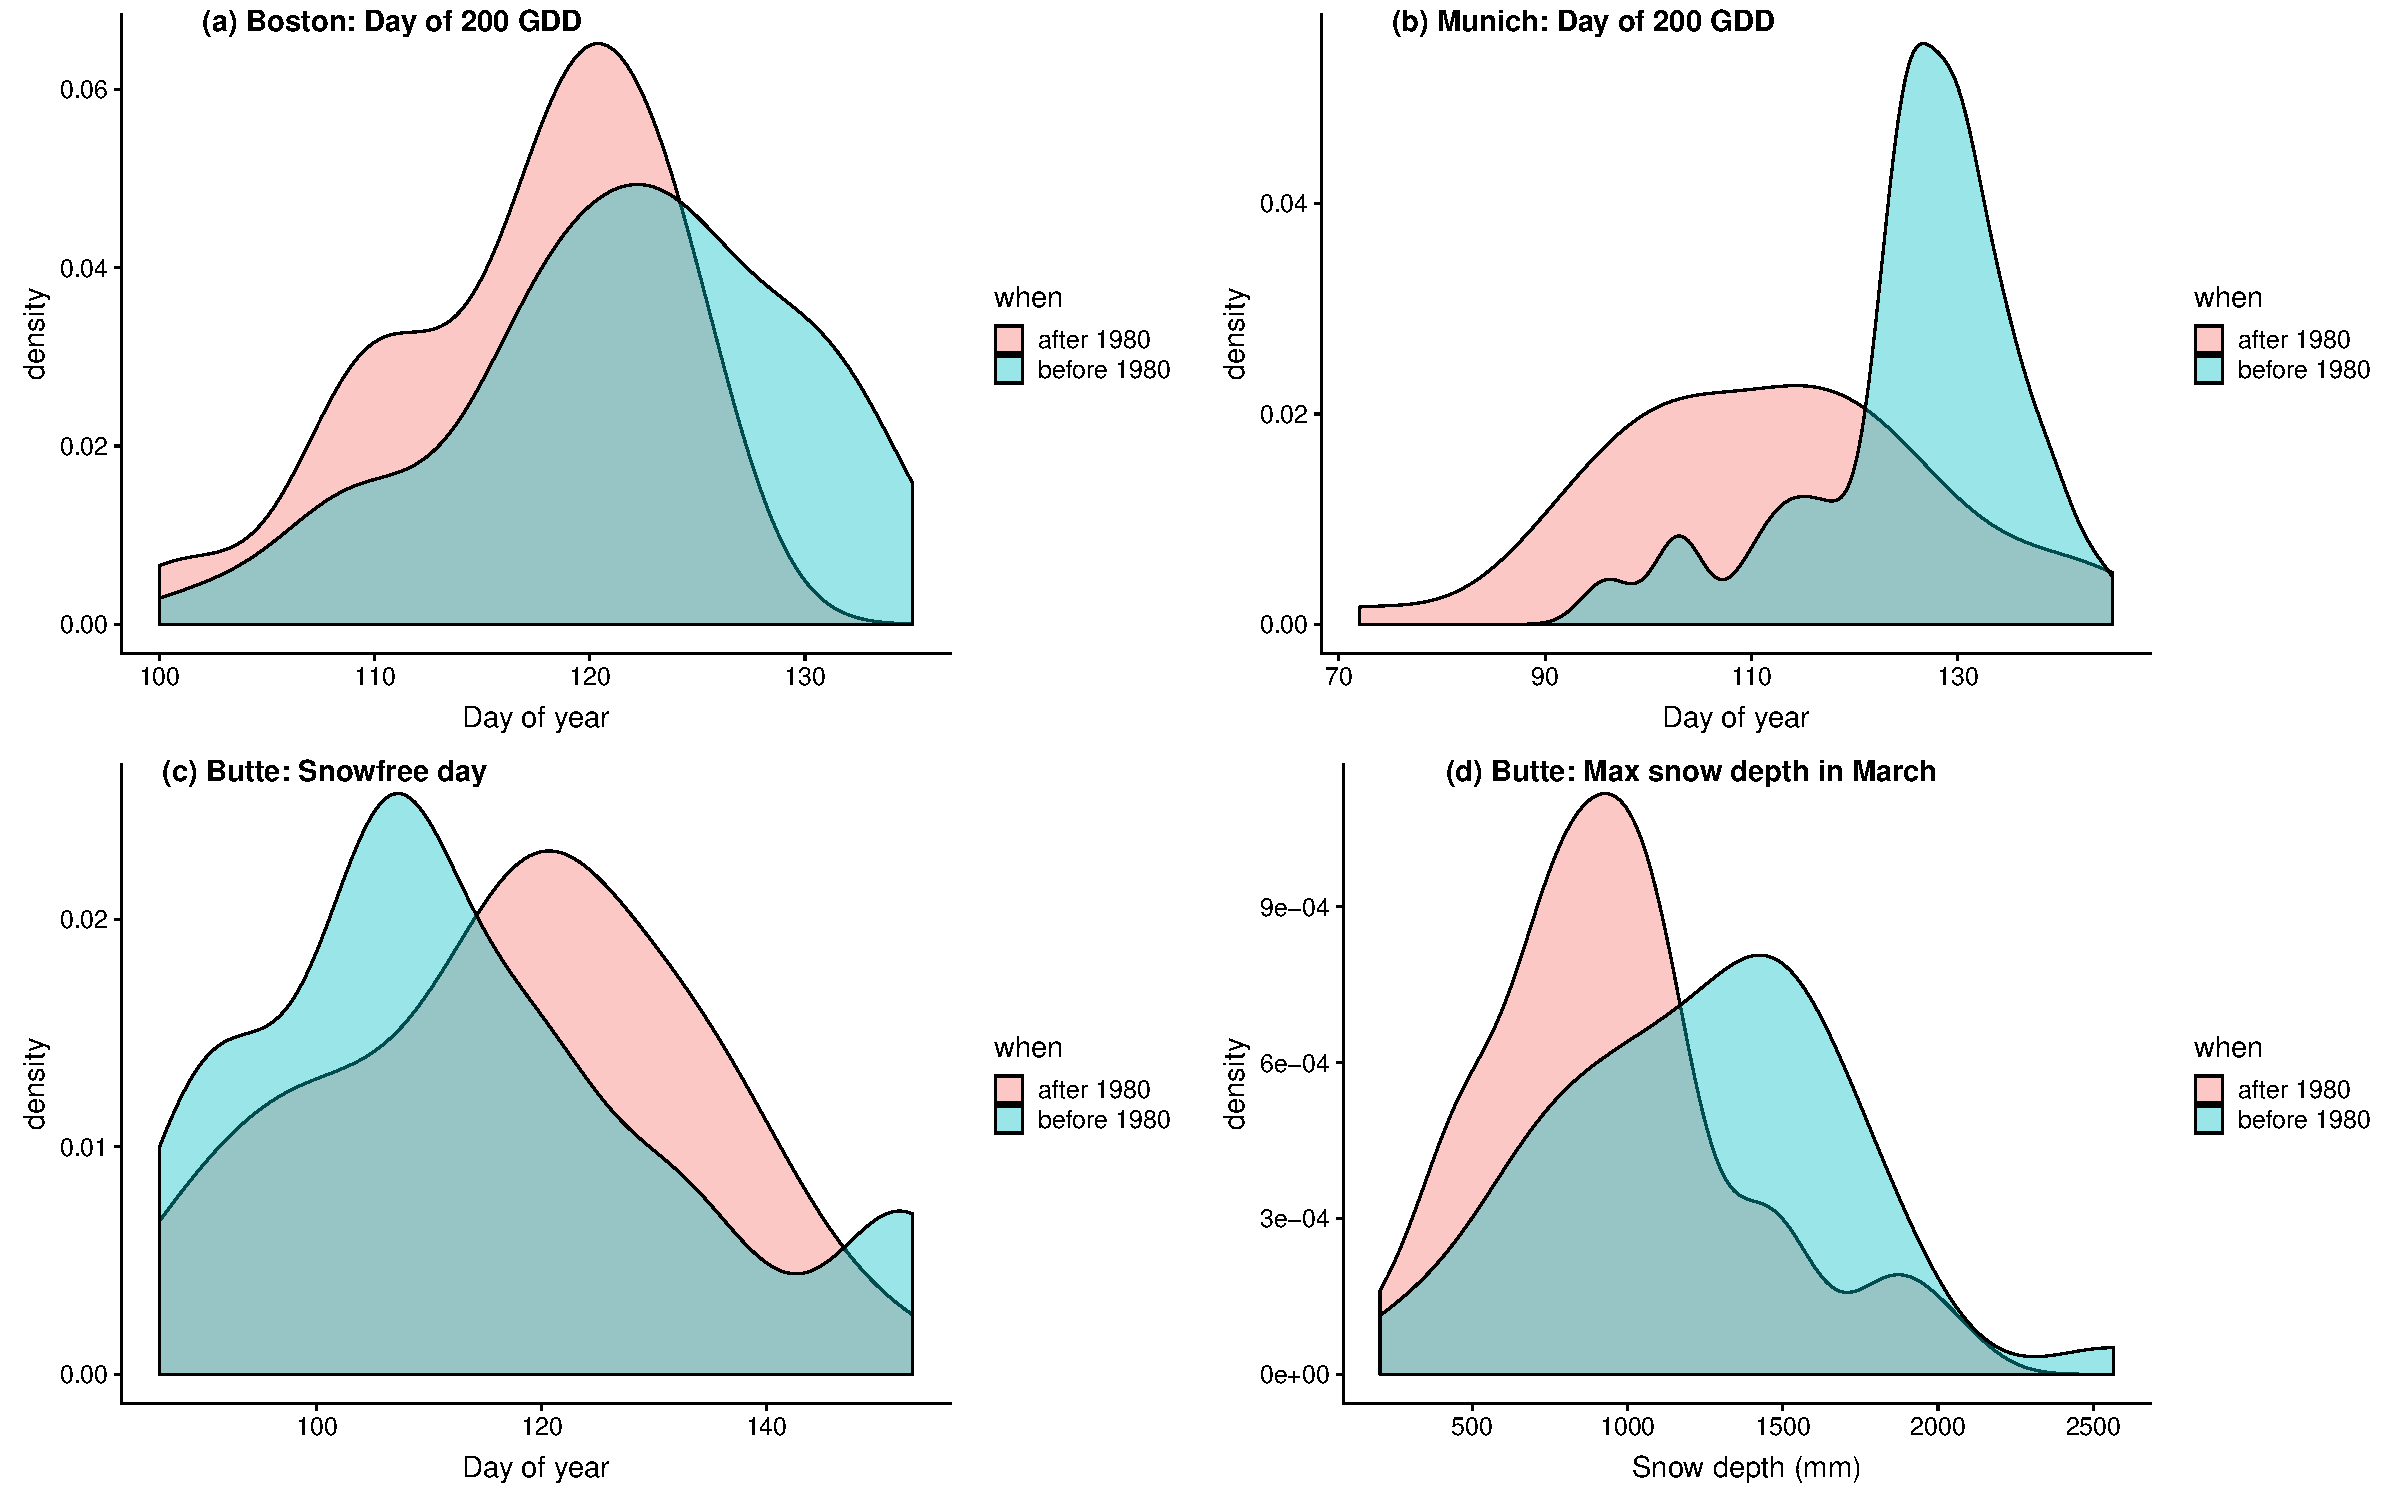
\includegraphics[width=1\textwidth]{..//..//..//R/graphs/otherdat/climdata.pdf}
\caption{Examples of non-stationarity in climate variables linked to environmental tracking: shifts before and after 1980 (a major change-point in climate for many regions) in several metrics related to the start of growing seasons (a-c) or resource pulse connected to growing season length (d). Density plots of day of 200 growing degree day units (a metric of thermal sum, here based on 0 degree base temperature using daily minima in $\degree$C) in Boston, MA, USA (a), and Munich, Germany (b), first snowfree day (followed by at least 9 snowfree days) in Crested Butte, CO, USA (c) and maximum snowdepth (mm) in March (often the month before the first snowfree day) in Crested Butte, CO, USA (d). Note that (c) and (d) are likely related, with lower snowpacks leading to an earlier first snowfree day. We selected sites that have been studied for plant phenological data and included at least 80 years of daily climate data from a Global Historical Climatology Network site; we subsetted data so that there were 40 years before and after 1980 for all sites.} %  (downloaded from \href{https://climexp.knmi.nl/})
 \label{fig:climdat}
\end{figure}

\begin{figure}[h!]
\centering
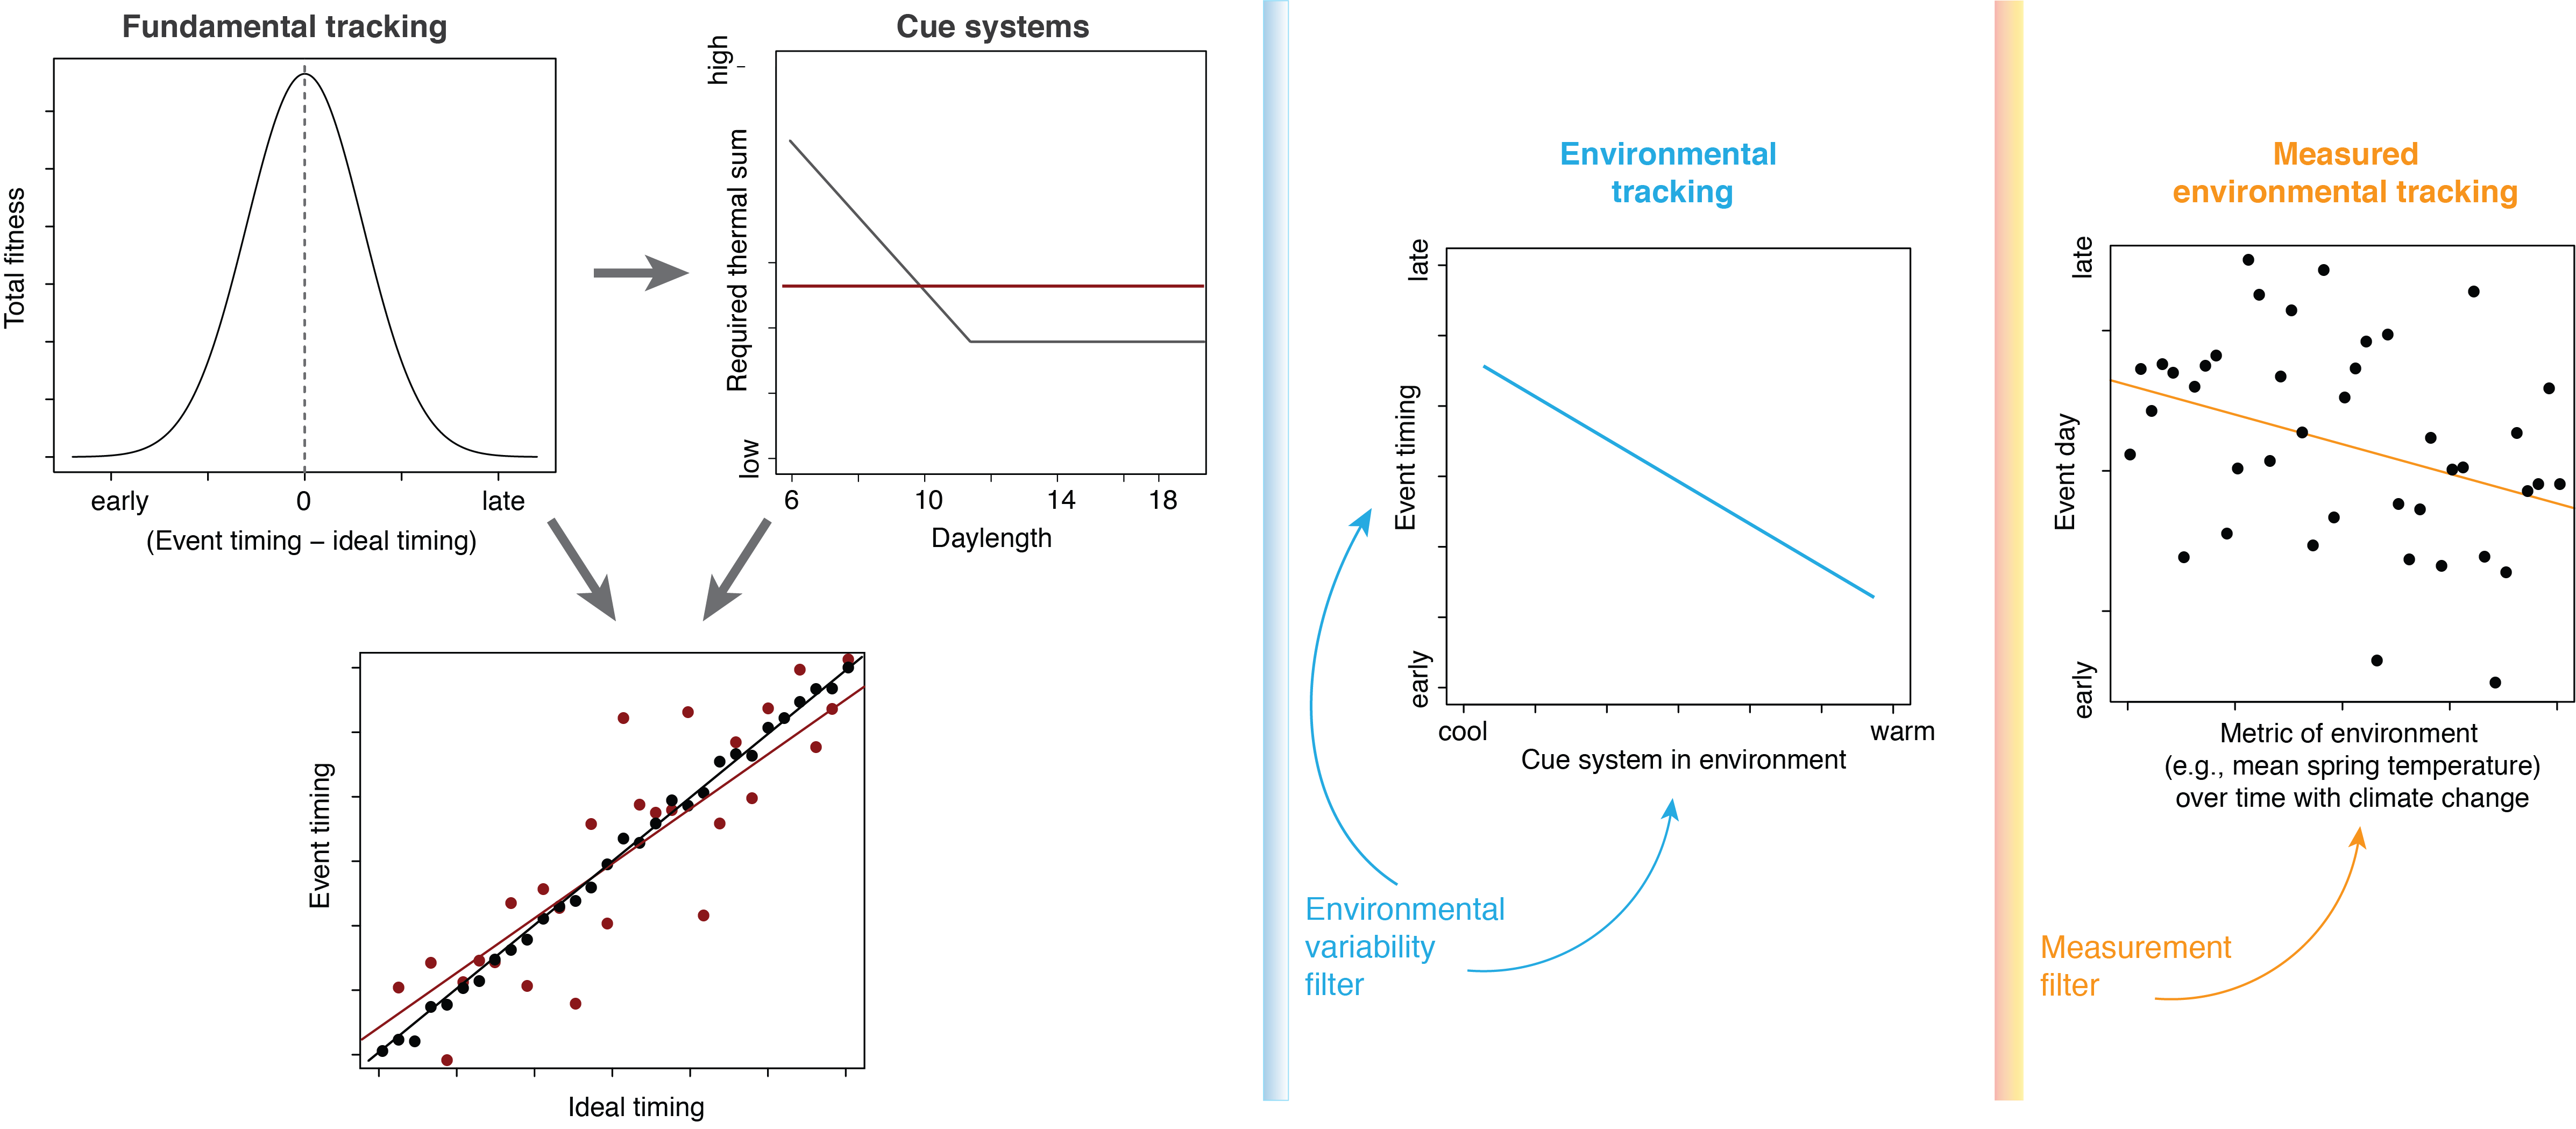
\includegraphics[width=1\textwidth]{..//..//..//R/graphs/conceptual/envtracking_define.png}
\caption{Defining tracking: Fundamental tracking (top left) represents how an organism matches the actual timing of a life history event to the timing that maximizes its fitness (i.e., ideal timing). Here, we show one conceptualization, where fitness declines as event timing moves away from the ideal timing, though realizations in nature may take diverse forms. The cue system is the physiological machinery that an organism uses to predict the ideal timing; we show one dependent only on daylength (red line: the event occurs when the organism's environment exceeds a certain daylength) and one that depends on a combination of daylength and thermal sums (navy line: the event occurs when the organism accumulates enough temperature for the current daylength). The skill of a cue system in predicting the ideal timing represents cue quality (bottom left). The combination of  environmental variability and an organism's cue system results in different event timings depending on the environment, what we define as environmental tracking (middle). Measured environmental tracking (right) depends both on environmental tracking and the metric(s) of the environment that researchers measure. } 
 \label{fig:defineET}
\end{figure}

\begin{figure}[h!]
\centering
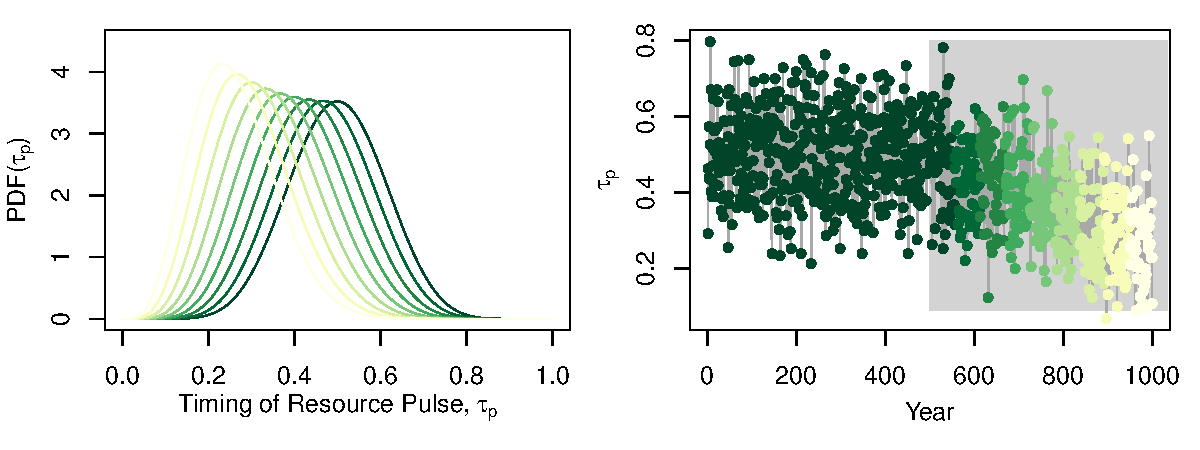
\includegraphics[width=1\textwidth]{..//..//..//R/graphs/modelruns/manuscript/modelsuppAlt.pdf}
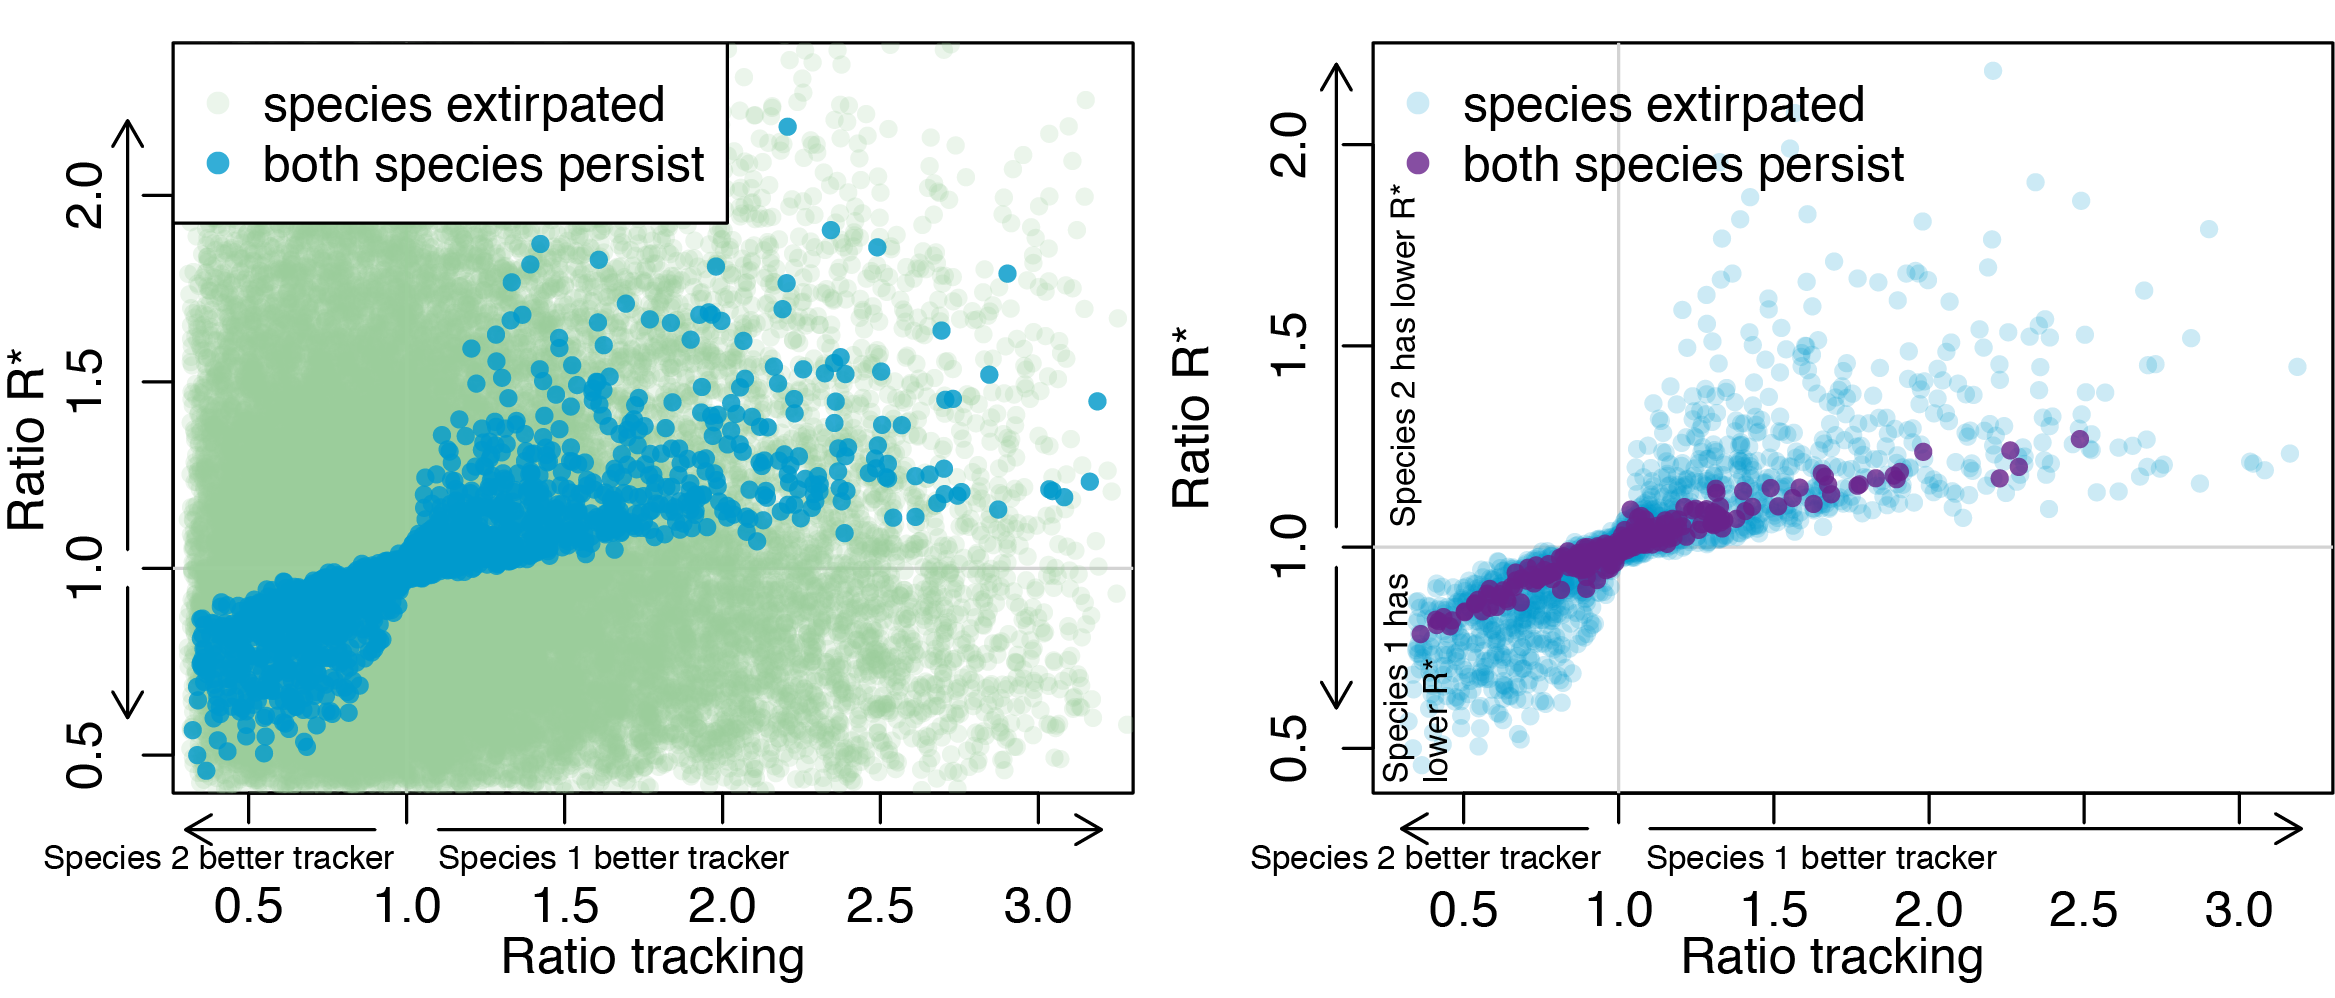
\includegraphics[width=0.96\textwidth]{..//..//..//R/graphs/modelruns/manuscript/alpharstar_2panelwide_adj.png}
\caption{Example of how non-stationarity can reshape communities in a simple model. We shifted the environment (top panels) by changing the timing of the resource pulse from a stationary period ($\tau_{p} \sim \beta(10,10)$ for the 500 years) to a nonstationary period ($\tau_{p}\sim \beta(5,15)$ over the 500 years), then examined outcomes for two-species communities (bottom panels) where tracking (X axis: species 1/species 2) trades off with $R^*$ (Y axis: species 1/species 2): each point represents one two-species community color-coded by whether both species persisted or one or more species was extirpated through 500 years of a stationary environment (bottom-left), followed by an additional 500 years of non-stationary environment (bottom-right, only two-species communities that persisted through the stationary period are shown).}
\label{fig:modelfig} 
\end{figure}

\begin{figure}[h!]
\centering
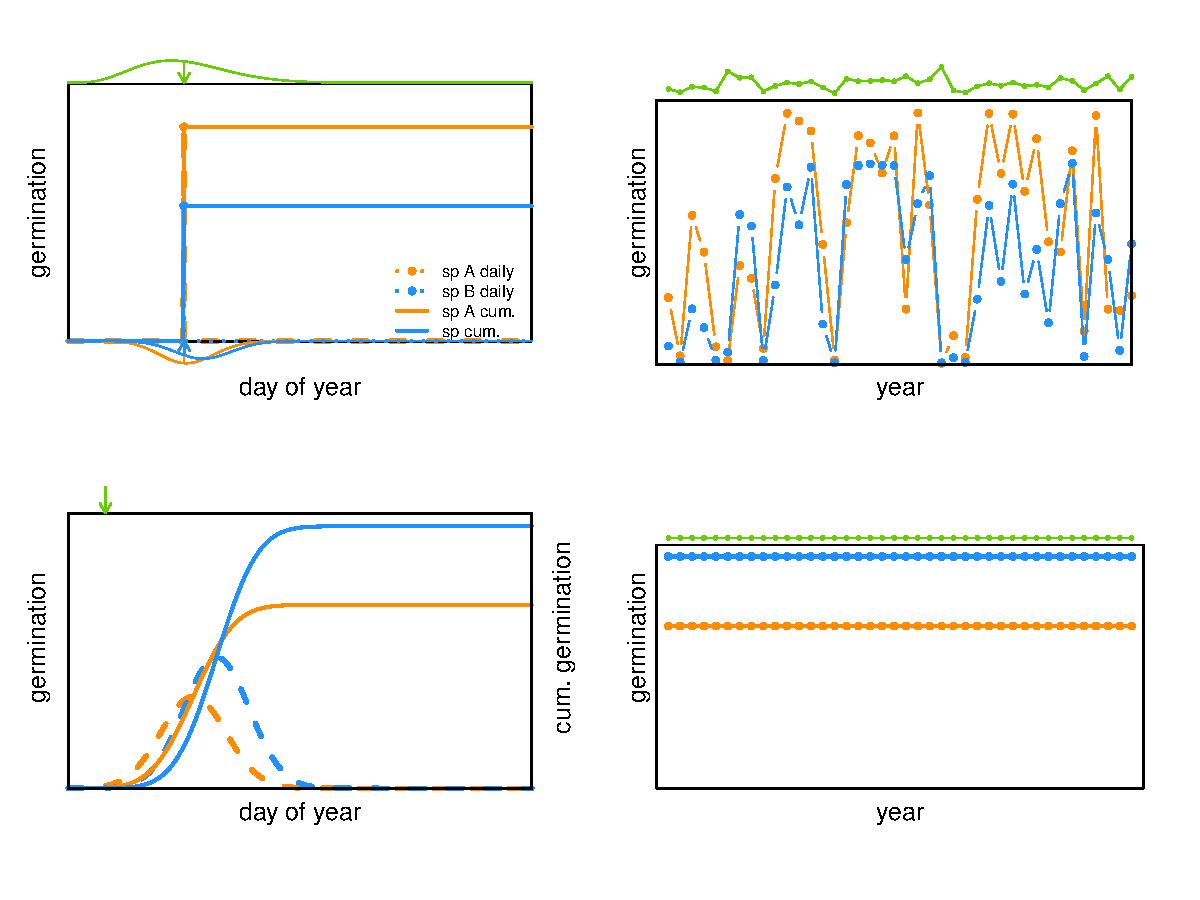
\includegraphics[width=1.1\textwidth]{..//..//..//R/graphs/conceptual/PriorityEff_BetHedge.pdf}
\caption{Tracking can be conceptualized as changes in priority effects or changes in storage effects.  In a priority effect model (A,B), the coexistence mechanism is a within-year tradeoff between, an early-germinating species that pre-empts resources (sp 1) and late-germinating species that is a superior resource competitor (sp 2) (A, where green arrow indicates the start of season); no between-year variation is required to maintain coexistence. In a storage effect model (C,D), variation in the timing of the start of season (indicated by the distribution in green, top of C) results results in differential species-response to the environment (illustrated by species-specific germination curves, bottom of C); this interannual variation in species-response to the environment (D)---along with a seedbank or other interannual storage mechanism---can maintain coexistence through reduced interspecific competition.}
\label{fig:conceptmodels} 
\end{figure}


%=======================================================================
% References
%=======================================================================
\clearpage
\newpage
\bibliography{/Users/Lizzie/Documents/git/bibtex/LizzieMainMinimal}
\bibliographystyle{/Users/Lizzie/Documents/git/bibtex/styles/ecolett.bst}


%=======================================================================
% Tables
%=======================================================================

%\begin{center}  
%\begin{table}
%\caption{Key differences between PWR and traditional PCMs such as PGLS.}
%\begin{tabular}{ | p{4cm} | p{5.5 cm} | p{5.5 cm} |}   \hline 
%& PWR & PCMs (e.g., PGLS) \\ \hline \hline
%Major goal & Study of evolution of correlation between variables across species & Study of evolution of correlation between variables across species\\ \hline
%\emph{Assumption 1:} Nature of correlation between two or more variables & Non-stationary (changes through phylogeny in a phylogenetically conserved fashion) & Stationary (constant) throughout phylogeny (all variation is noise) \\ \hline
%\emph{Assumption 2:} Completeness of variables & Substitutes phylogeny for variables (simple or complex) not in the model that interact with variables in the model & Assumes variables in model are primary drivers of correlational relationship \\ \hline
%Inferential mode & Usually exploratory & Hypothesis testing (statistical significance)\\ \hline
%Outputs & Coefficients of regression changing through the phylogeny & p-value and single set of coefficients presumed to apply to entire phylogeny with their confidence intervals\\ \hline

%Method to avoid overfitting & Cross-validation (boot-strapped determination of optimal band-width for accurate prediciton of hold-outs) & Exact analytical model of errors and degrees of freedom\\ \hline \hline
%\end{tabular}
%\end{table}
%\end{center}

%=======================================================================
% Paste in revision letter here to make line numbers work
%=======================================================================
\nolinenumbers
\newpage
\setcounter{page}{1}

\end{document}
%%%%%%%%%%%%%%%%%%%%%%%%%%%%%%%%%%%%%%%%%%%%%%%%%%%%%%%%%%%%%%%%%%%%%%%%

\begin{enumerate}
\item Figure for ... The shape of this underlying distribution varies across systems and in how it is measured---the amount of rainfall in semi-arid systems is often highly skewed compared the thermal sum of many temperate growing season
\item With climate change, warming has increased mean temperatures over time, with minimum temperatures generally increasing mre than maximum---this results in an underlying distribution for daily temperature where the mean is both increased through time and the variance is decreasing (Munich garden? Maybe add San Dieg precip example?
\item Real-world data showing stat/non-stationarity in environment (ideally $\tau_{p}$) 
\item Real-world data showing tracking (and less tracking)
\item $\tau_{i}$ vs. R* trade-off and histogram of persisting $\tau_i$ under stat/nonstat $\tau_{p}$ environment
\item alpha vs.$\tau_i$ trade-off and histogram of persisting alpha under stat/nonstat $\tau_{p}$ environment
\item alpha vs. R* trade-off and histogram of persisting alpha under stat/nonstat $\tau_{p}$ environment
\item (Scratch this one: we're pretty sure it required a crappy $\tau_i$ to survive the initial stationary period, then be favored in second time period and we're not so sure crappy $\tau_i$ species survive the initial stationary period) time-series of one run showing years where $\tau_i$ of one species is close to $\tau_{p}$ and other years where $\tau_i$ of other species is close to $\tau_{p}$ (and show this shift under nonstat)
\item non-stationarity in $R0$ and $\tau_{p}$
\end{enumerate}


%=======================================================================
% to-do listing
%=======================================================================

\listoftodos

%=======================================================================
\section*{Other loose ends}
%=======================================================================

% Old hypothesis: Without tracking we may predict benefits to early-colonizers decline with earlier seasons. As start-date moves earlier, early folks lose benefit (assuming they tend to often go at optimum time) and you get more late folks. Late species may be less different than one another---and less responsive to environment. Early folks, effectively, become more similar to environment. 

% Environmental variability means many species should benefit from tracking their environment. We focus here on environmental tracking through time (often referred to below as `tracking') rather than through space because of its well-established links to individual-level physiology, yielding a more robust understanding of what environmental cues determine tracking \citep{chuineJTB,Chew:2012pd}, and because it has been repeatedly linked to performance and other fitness-related metrics. Temporal environmental cues, however, are often linked to species' ranges \citep{Morin:2008vp,arabid2011}, thus we expect much of this work could extend to environmental tracking through space. 
% Definition of tracking: correlation between a recurring biological event and something else in its environment

Many (or potentially all) species use abiotic cues to trigger major phenological events. These cues in turn result in different rates of tracking. At one extreme, some cues yield a fixed timing, resulting in no tracking over time. A common example of a fixed cue is photoperiod, which results in event timing that is constant across years (but variable across space, allowing---for example, later timings poleward for spring events) and appears widespread for some insect emergence and for fall senescence of many trees \citep{Denlinger2017,lechowiczbook2002}. Fixed timings are perhaps the simplest option and may be efficient for events where there is low predictability, low variability, or low costs to being too late or early. In cases where there is a high cost to mis-timing an event across a variable environment, cues that yield more variability in timing are far more prevalent and usually rely on climate. Temperature is a widespread cue for start of season events with many organisms needing a certain thermal sum to start visible growth. Such a cue has the benefit of shifting the date of an event early or late, depending on climatic conditions, each year, but may be a poor cue in years with aberrant events (e.g., a late frost). In most systems, species must use environmental cues such as temperature to forecast the ideal date for an event---a date which is only obvious in retrospect. ...  Measuring tracking depends on many factors (see Box `What underlies variability in species tracking?'). 






